% Apresentação breve: análise dos resultados dos modelos (Brasil, regiões e UFs).
% Figuras geradas por gerar_figuras.py. Compile com pdflatex ou tectonic nesta pasta.
\documentclass[10pt,aspectratio=169]{beamer}

\usepackage[utf8]{inputenc}
\usepackage[T1]{fontenc}
\usepackage[brazil]{babel}
\usepackage{lmodern}
\usepackage{graphicx}
\usepackage{booktabs}
\usepackage{amsmath}
\usepackage{xcolor}
\usepackage{tikz}
\usetikzlibrary{positioning,arrows.meta,calc}
\usepackage[most]{tcolorbox}

% ---------------------------------------------------------------
% Cores
% ---------------------------------------------------------------
\definecolor{pucnavy}{RGB}{7,27,51}
\definecolor{pucblue}{RGB}{18,100,163}
\definecolor{puccyan}{RGB}{50,180,200}
\definecolor{pucorange}{RGB}{246,160,65}
\definecolor{pucgray}{RGB}{96,112,138}
\definecolor{puclight}{RGB}{238,244,250}

% ---------------------------------------------------------------
% Aparência geral
% ---------------------------------------------------------------
\setbeamertemplate{navigation symbols}{}
\setbeamersize{text margin left=1cm,text margin right=1cm}
\setbeamercolor{structure}{fg=pucblue}
\setbeamercolor{frametitle}{fg=pucnavy,bg=white}
\setbeamerfont{frametitle}{series=\bfseries,size=\Large}
\setbeamercolor{normal text}{fg=pucnavy,bg=white}
\setbeamercolor{block title}{fg=white,bg=pucblue}
\setbeamercolor{block body}{fg=pucnavy,bg=puclight}
\setbeamertemplate{itemize item}{\color{pucorange}\small$\blacktriangleright$}
\setbeamertemplate{enumerate item}{\color{pucblue}\bfseries\insertenumlabel.}
\setlength{\leftmargini}{1.2em}

% Título do frame com marcador laranja e filete
\setbeamertemplate{frametitle}{%
  \vskip.3cm
  \begin{beamercolorbox}[wd=\paperwidth,leftskip=1cm,rightskip=1cm]{frametitle}
    \usebeamerfont{frametitle}%
    {\color{pucorange}\rule[-.2em]{3pt}{1.1em}}\hspace{.3cm}\insertframetitle
  \end{beamercolorbox}
  \vskip.1cm
  \begin{beamercolorbox}[wd=\paperwidth,leftskip=1cm,rightskip=1cm]{frametitle}
    {\color{pucblue!20}\rule{\dimexpr\paperwidth-2cm\relax}{.6pt}}
  \end{beamercolorbox}
  \vskip.05cm
}

% Rodapé com barra de progresso
\setbeamertemplate{footline}{%
  \begin{tikzpicture}
    \useasboundingbox (0,0) rectangle (\paperwidth,.7cm);
    \fill[pucblue!10] (0,.66cm) rectangle (\paperwidth,.7cm);
    \fill[pucorange] (0,.66cm) rectangle
      ({\paperwidth*\insertframenumber/\inserttotalframenumber},.7cm);
    \node[anchor=west,text=pucgray,font=\scriptsize] at (1cm,.3cm)
      {IND2616: Séries Temporais \quad|\quad PUC-Rio};
    \node[anchor=east,text=pucgray,font=\scriptsize] at (\paperwidth-1cm,.3cm)
      {\insertframenumber\,/\,\inserttotalframenumber};
  \end{tikzpicture}%
}

% ---------------------------------------------------------------
% Componentes
% ---------------------------------------------------------------
% Cartão claro com borda lateral azul
\newtcolorbox{cartao}[1][]{enhanced,colback=puclight,colframe=puclight,
  boxrule=0pt,arc=2mm,left=8pt,right=8pt,top=6pt,bottom=6pt,
  borderline west={3pt}{0pt}{pucblue},before upper=\raggedright,#1}

% Caixa de mensagem principal (fundo escuro)
\newtcolorbox{mensagem}[1][]{enhanced,colback=pucnavy,colframe=pucnavy,
  coltext=white,boxrule=0pt,arc=2mm,left=10pt,right=10pt,top=7pt,bottom=7pt,#1}

% Número em destaque
\newcommand{\numero}[3][\LARGE]{%
  \begin{cartao}[top=4pt,bottom=4pt]
    {\color{pucblue}#1\bfseries #2}\par\vspace{1pt}
    {\footnotesize #3}
  \end{cartao}}

% Etiqueta arredondada
\newcommand{\pill}[2][pucorange]{%
  \tikz[baseline=(p.base)]\node[fill=#1,text=white,rounded corners=7pt,
    inner xsep=5pt,inner ysep=2pt,font=\footnotesize\bfseries](p){#2};}

% Rótulo de seção dentro do slide
\newcommand{\rotulo}[1]{{\color{pucblue}\small\bfseries\MakeUppercase{#1}}\par\vspace{3pt}}

% Nota de rodapé do slide
\newcommand{\nota}[1]{{\color{pucgray}\scriptsize #1}}


\graphicspath{{figuras/}}
\title{Análise de resultados dos modelos}
\author{Thiago Paes \and Joan Souza \and Matheus Accioly \and Isabelle Gagno}
\date{Novembro de 2026}

\begin{document}

% ===============================================================
\begin{frame}[plain]
  \begin{tikzpicture}[remember picture,overlay]
    \fill[pucnavy] (current page.south west) rectangle (current page.north east);
    \fill[pucblue,opacity=.35] ([xshift=-.6cm,yshift=.4cm]current page.south east) circle (4.2cm);
    \fill[puccyan,opacity=.22] ([xshift=-2.6cm,yshift=-.6cm]current page.south east) circle (2.4cm);
    \fill[pucorange] (current page.north west) rectangle ([xshift=.25cm]current page.south west);
    \node[anchor=north west,text width=11.3cm,align=left,inner sep=0pt]
      at ([xshift=1.4cm,yshift=-1.2cm]current page.north west) {%
      {\color{puccyan}\large\bfseries IND2616: Séries Temporais}\par\vspace{.6cm}
      {\color{white}\fontsize{24}{29}\selectfont\bfseries
        Previsão de internações por VSR: análise dos resultados\par}
      \vspace{.4cm}
      {\color{white!78!pucnavy}\large Desempenho da política final em Brasil, regiões e UFs.\par}
      \vspace{.45cm}
      {\color{pucorange}\rule{2.2cm}{2pt}}\par\vspace{.3cm}
      {\color{white}\normalsize Thiago Paes \quad Joan Souza \quad Matheus Accioly \quad Isabelle Gagno\par}
      \vspace{.15cm}
      {\color{white!65!pucnavy}\small Mestrado PUC-Rio \quad|\quad Prof. Fernando Cyrino
        \quad|\quad Novembro de 2026\par}
    };
  \end{tikzpicture}
\end{frame}

% ===============================================================
\begin{frame}{O que está sendo avaliado}
  \begin{columns}[T,onlytextwidth]
    \begin{column}{.5\textwidth}
      \rotulo{Desenho}
      \begin{itemize}
        \item 33 séries: Brasil, 5 regiões e 27 UFs.
        \item 58 origens expansivas, sem vazamento (dez/2021 a abr/2026).
        \item Horizontes de 1, 4, 8 e 13 semanas.
        \item MASE: erro dividido pela escala do ingênuo sazonal de cada série; compara UF pequena com Brasil.
      \end{itemize}
    \end{column}
    \begin{column}{.46\textwidth}
      \rotulo{Duas previsões comparadas}
      \begin{cartao}
        \textbf{Base V2}: previsões independentes por série\par
        \footnotesize Saem diretamente dos modelos estatísticos. Não somam entre níveis.
      \end{cartao}
      \vspace{2pt}
      \begin{cartao}
        \textbf{Política final}: Base V2 + reconciliação\par
        \footnotesize Os mesmos modelos, ajustados pelo MinT para que UFs somem regiões e Brasil, sem negativos.
      \end{cartao}
      \nota{O MinT não é um modelo de previsão: ele só ajusta previsões que já existem.}
    \end{column}
  \end{columns}
\end{frame}

% ===============================================================
\begin{frame}{Como a previsão final é construída}
  \footnotesize
  \centering
  \begin{tabular}{lll}
    \toprule
    & \textbf{1 e 4 semanas} & \textbf{8 e 13 semanas} \\
    \midrule
    Passo 1, Brasil e 5 regiões & ETS amortecido (Holt-Winters) & Ingênuo sazonal \\
    Passo 1, 27 UFs & Ingênuo (repete a última semana) & Ingênuo sazonal \\
    Passo 2, reconciliação & MinT não negativo & Nenhuma (já soma) \\
    \bottomrule
  \end{tabular}\par\vspace{6pt}
  \vspace{-4pt}
  \begin{tikzpicture}[
      caixa/.style={draw=pucblue,fill=puclight,rounded corners=2mm,align=center,
        text width=3.1cm,minimum height=1cm,font=\scriptsize},
      seta/.style={-{Stealth},thick,pucorange}]
    \node[caixa] (ets) at (0,.75) {\textbf{ETS amortecido}\\Brasil + 5 regiões\\6 previsões};
    \node[caixa] (ing) at (0,-.75) {\textbf{Ingênuo}\\27 UFs\\27 previsões};
    \node[caixa,text width=3.6cm,fill=pucnavy,text=white,draw=pucnavy] (mint) at (4.6,0)
      {\textbf{MinT não negativo}\\pesa cada previsão pela confiabilidade histórica (covariância dos erros) e exige UFs $\ge 0$};
    \node[caixa] (uf) at (9.2,.75) {\textbf{27 UFs}\\reconciliadas};
    \node[caixa] (agg) at (9.2,-.75) {\textbf{Regiões e Brasil}\\= soma das UFs};
    \draw[seta] (ets) -- (mint); \draw[seta] (ing) -- (mint);
    \draw[seta] (mint) -- (uf); \draw[seta] (uf) -- (agg);
  \end{tikzpicture}\par\vspace{4pt}
  \raggedright\footnotesize
  As 33 previsões do passo 1 discordam entre si: o ETS do Brasil não é igual à soma dos ingênuos das UFs. O MinT busca os valores mais próximos de todas elas que somam corretamente. Em 8 e 13 semanas, copiar a temporada anterior em todas as séries já soma, e o MinT devolve os mesmos números.
\end{frame}

% ===============================================================
\begin{frame}{Qual ETS? Seleção entre três candidatos}
  \scriptsize
  \centering
  \begin{tabular}{lccccl}
    \toprule
    Candidato & Tendência & MASE $h=1$ & MASE $h=4$ & Negativas$\to$0 ($h=4$) & Situação \\
    \midrule
    Sazonal aditivo & nenhuma & 0,551 & 1,511 & 2,9\% & comparado \\
    Tendência aditiva & aditiva & 0,541 & 1,442 & 12,9\% & excluído \\
    \textbf{Tendência amortecida} & \textbf{aditiva amortecida} & \textbf{0,507} & \textbf{1,311} & 6,0\% & \textbf{selecionado} \\
    \bottomrule
  \end{tabular}\par
  \nota{Todos com sazonalidade aditiva de 52 semanas. MASE médio de Brasil e regiões, 348 avaliações por célula. Negativas$\to$0: previsões negativas truncadas em zero.}\par\vspace{6pt}
  \begin{columns}[T,onlytextwidth]
    \begin{column}{.52\textwidth}
      \rotulo{O modelo selecionado}
      \begin{itemize}
        \item Holt-Winters aditivo com tendência amortecida, equivalente às previsões pontuais do ETS(A,Ad,A).
        \item Período sazonal de 52 semanas e inicialização heurística (\texttt{statsmodels} \texttt{ExponentialSmoothing}).
        \item Reajustado em cada uma das 58 origens: 348 de 348 ajustes convergiram.
      \end{itemize}
    \end{column}
    \begin{column}{.44\textwidth}
      \rotulo{Por que este}
      \begin{itemize}
        \item Menor MASE em 1 e 4 semanas para Brasil e regiões.
        \item A tendência sem amortecimento extrapola quedas e gera muitas previsões negativas, corrigidas para zero.
        \item O amortecimento faz a tendência perder força com o horizonte.
      \end{itemize}
    \end{column}
  \end{columns}
\end{frame}

% ===============================================================
\begin{frame}{Critério de comparação: a política supera os baselines?}
  \centering
  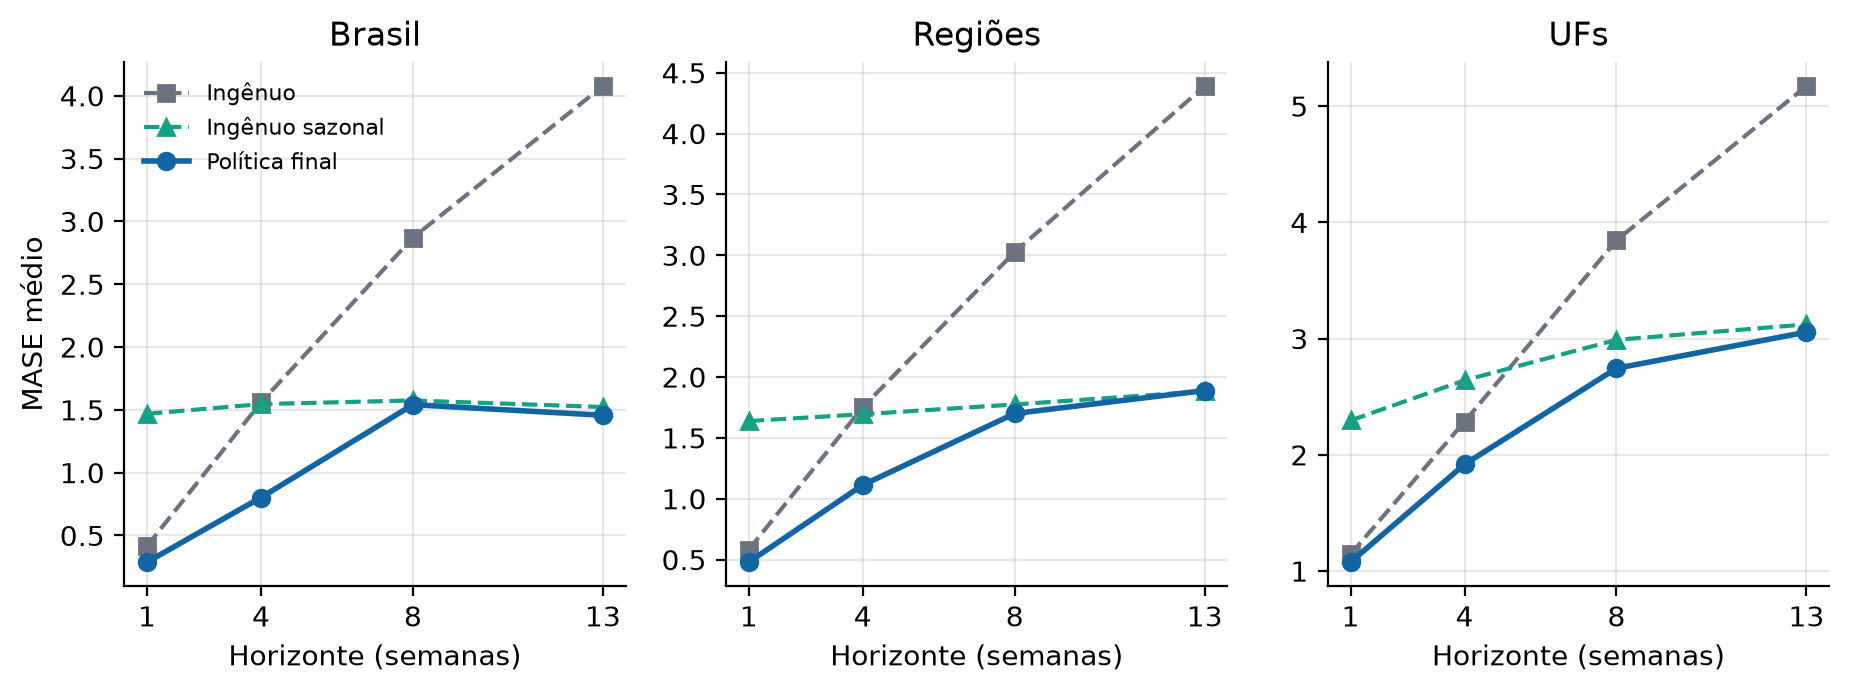
\includegraphics[width=.85\textwidth]{baselines_vs_politica.png}\par\vspace{2pt}
  \footnotesize
  \begin{tabular}{lccc}
    \toprule
    MASE: política vs.\ melhor baseline & Brasil & Regiões & UFs \\
    \midrule
    $h=1$ (vs.\ ingênuo) & 0,332 vs.\ 0,415 & 0,534 vs.\ 0,582 & 1,133 vs.\ 1,145 \\
    $h=4$ (vs.\ melhor ingênuo) & 1,202 vs.\ 1,546 & 1,417 vs.\ 1,694 & 2,211 vs.\ 2,285 \\
    $h=8$ e $13$ & \multicolumn{3}{c}{iguais: a política \emph{é} o ingênuo sazonal} \\
    \bottomrule
  \end{tabular}
\end{frame}

% ===============================================================
\begin{frame}{Visão geral: o erro cresce com o horizonte e cai com a agregação}
  \centering
  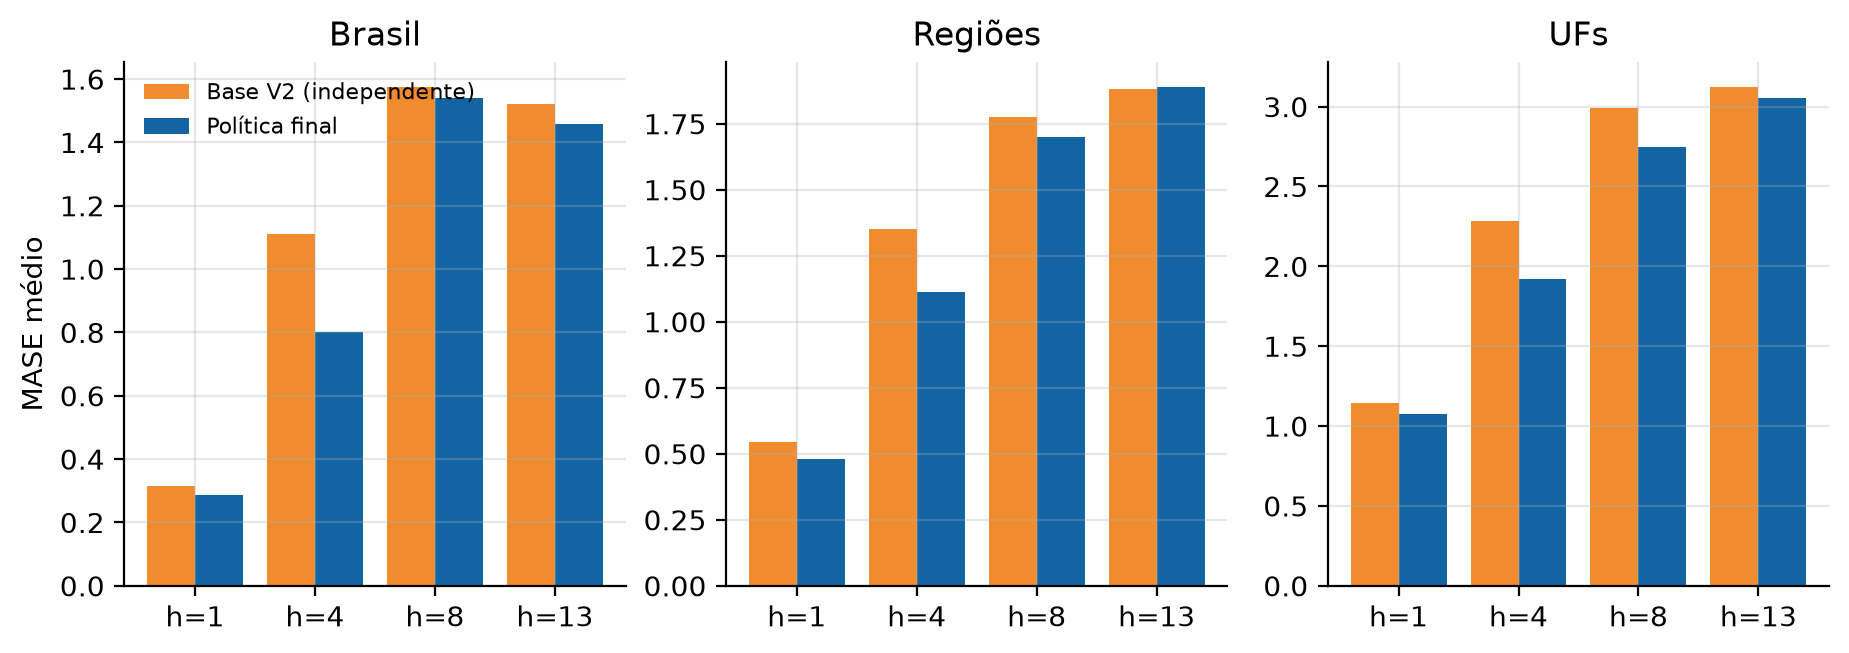
\includegraphics[width=.85\textwidth]{mase_nivel_horizonte.png}\par\vspace{4pt}
  \begin{columns}[T,onlytextwidth]
    \begin{column}{.32\textwidth}\small Brasil: a reconciliação custa pouco (0,315 $\to$ 0,332 em $h=1$).\end{column}
    \begin{column}{.32\textwidth}\small Regiões: ganho leve em $h=1$, perda em $h=4$.\end{column}
    \begin{column}{.32\textwidth}\small UFs: ganho em $h=1$ e $h=4$ (2,285 $\to$ 2,211).\end{column}
  \end{columns}
\end{frame}

% ===============================================================
\begin{frame}{Brasil: observado vs.\ política final, por horizonte}
  \begin{columns}[T,onlytextwidth]
    \begin{column}{.68\textwidth}
      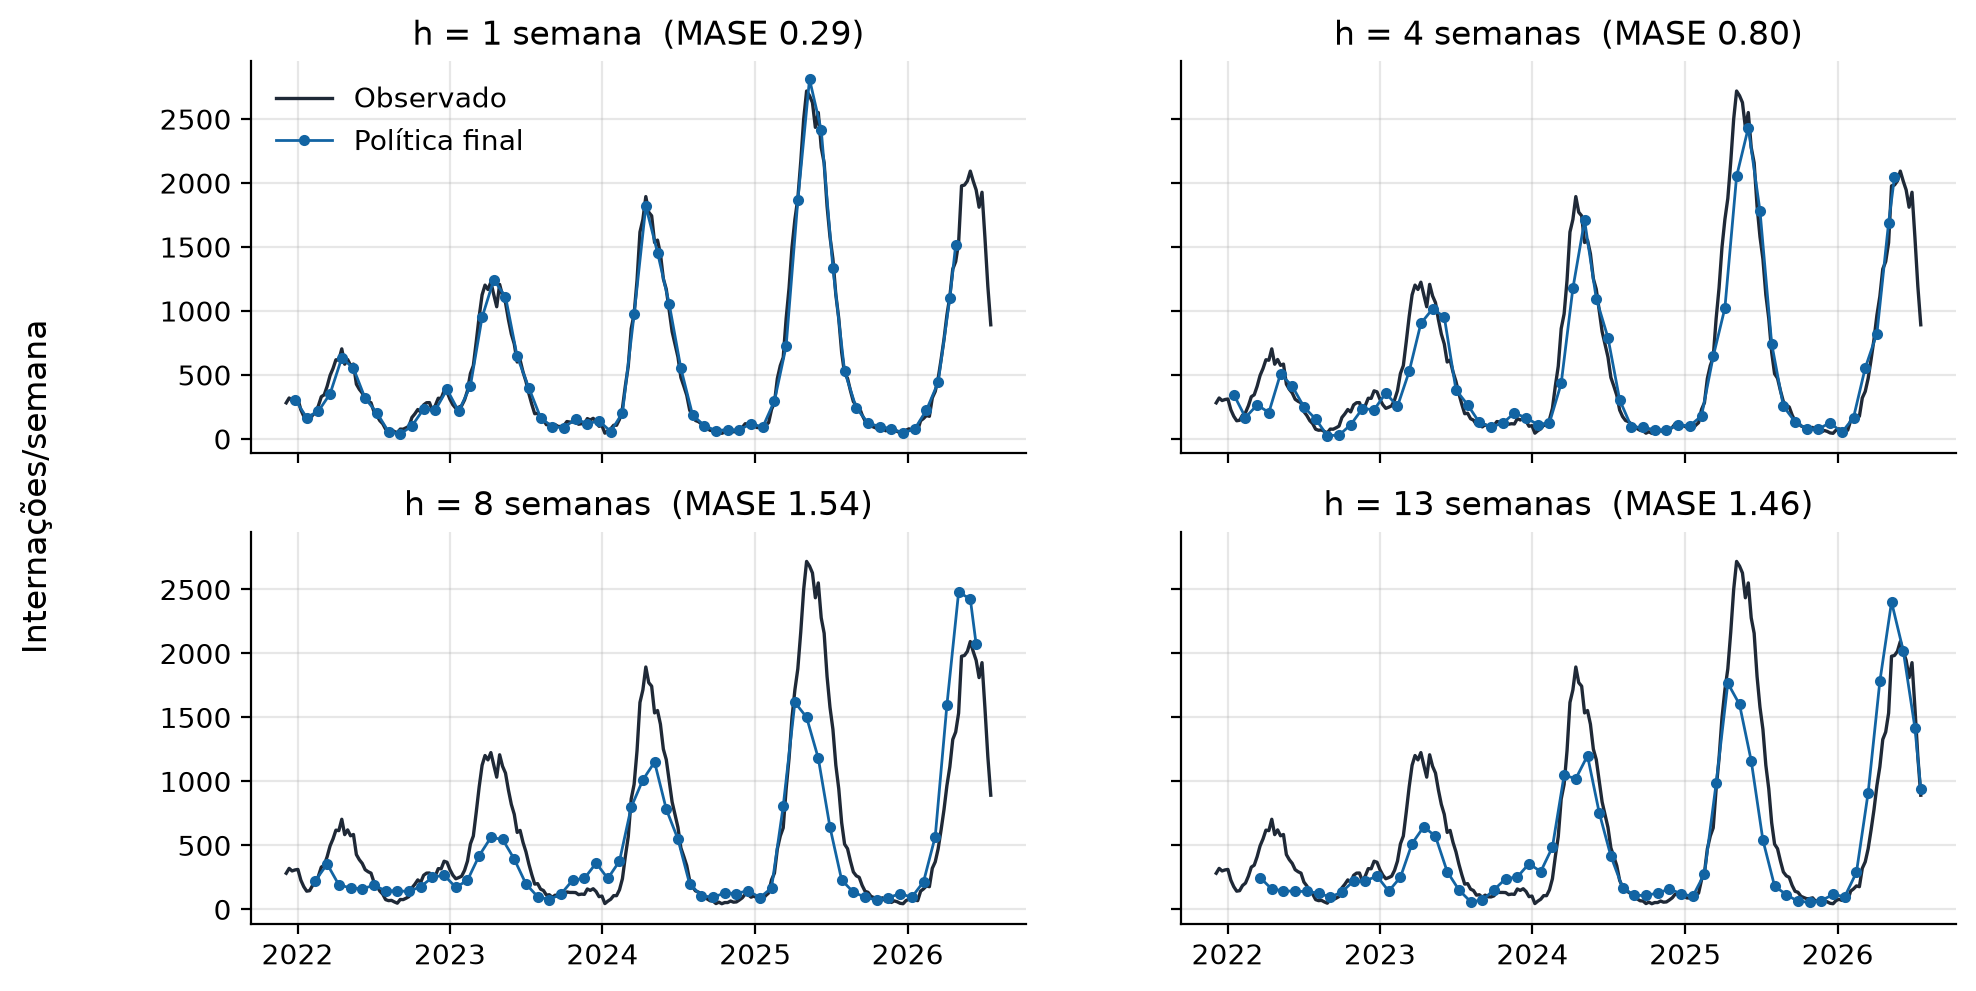
\includegraphics[width=\textwidth]{brasil_obs_vs_prev.png}
    \end{column}
    \begin{column}{.3\textwidth}
      \small
      \begin{itemize}
        \item $h=1$: acompanha a curva quase exatamente (MASE 0,33).
        \item $h=4$: forma correta, mas atrasa e exagera picos (2025: $\approx$3.200 previsto vs.\ 2.700).
        \item $h=8$ e $13$: aqui a política é o ingênuo sazonal, que repete a temporada anterior; acerta o calendário, erra a amplitude quando a onda muda de tamanho.
      \end{itemize}
    \end{column}
  \end{columns}
\end{frame}

% ===============================================================
\begin{frame}{Regiões: onde a política acerta e onde perde}
  \centering
  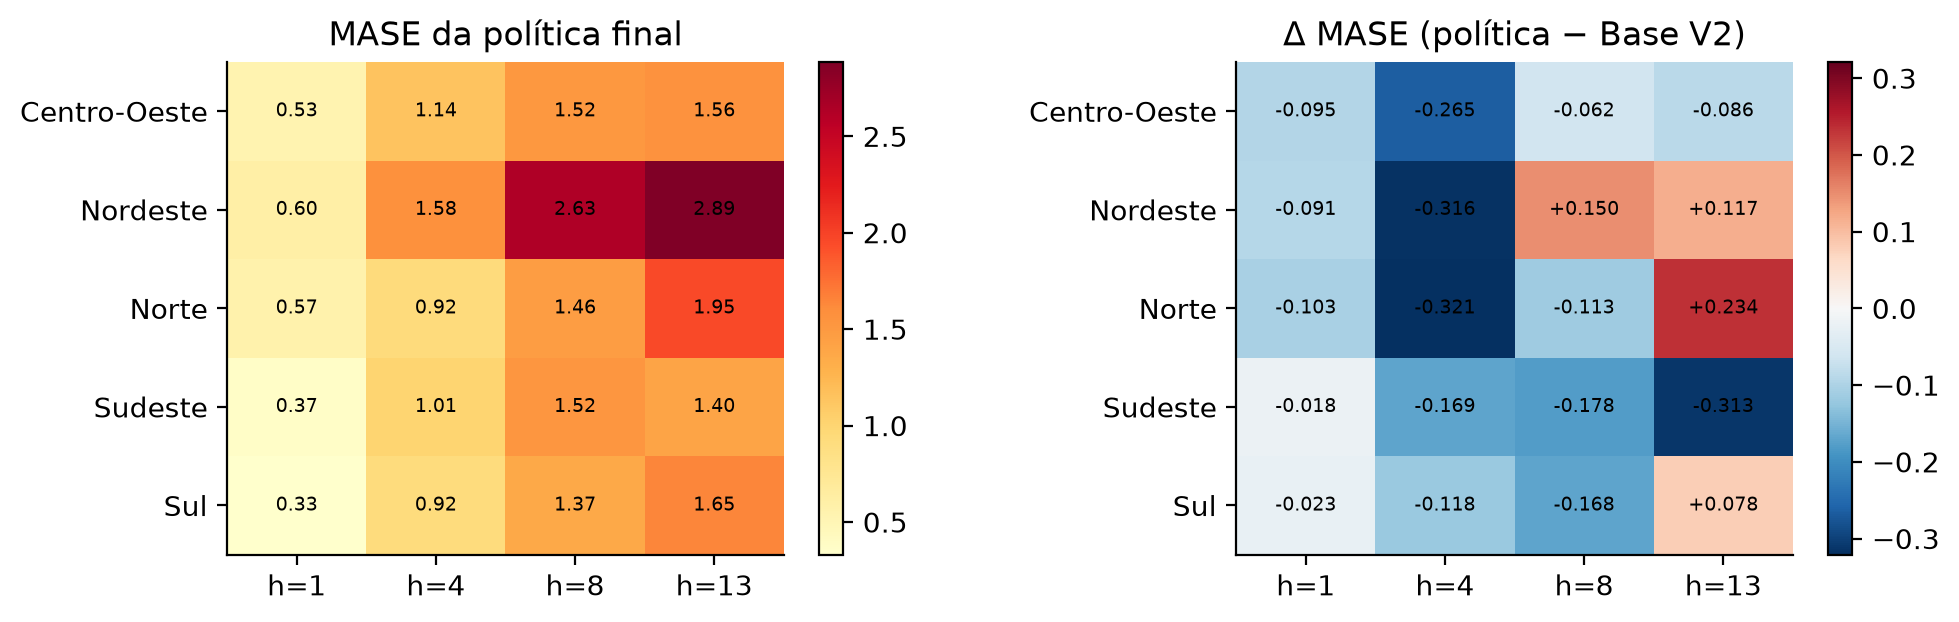
\includegraphics[width=\textwidth]{regioes_mase.png}\par\vspace{4pt}
  \begin{columns}[T,onlytextwidth]
    \begin{column}{.48\textwidth}\small
      Sudeste e Sul são as mais previsíveis em $h=1$ (0,34 e 0,37). O Nordeste é a mais difícil em todos os horizontes (2,77 em $h=13$), com picos mais tardios e variáveis.
    \end{column}
    \begin{column}{.48\textwidth}\small
      Em $h=1$ o MinT melhora 3 de 5 regiões; em $h=4$ só o Norte melhora. Em $h\ge8$ não há diferença: a Base V2 já é coerente.
    \end{column}
  \end{columns}
\end{frame}

% ===============================================================
\begin{frame}{Regiões: previsões de 4 semanas ao longo das origens}
  \begin{columns}[T,onlytextwidth]
    \begin{column}{.66\textwidth}
      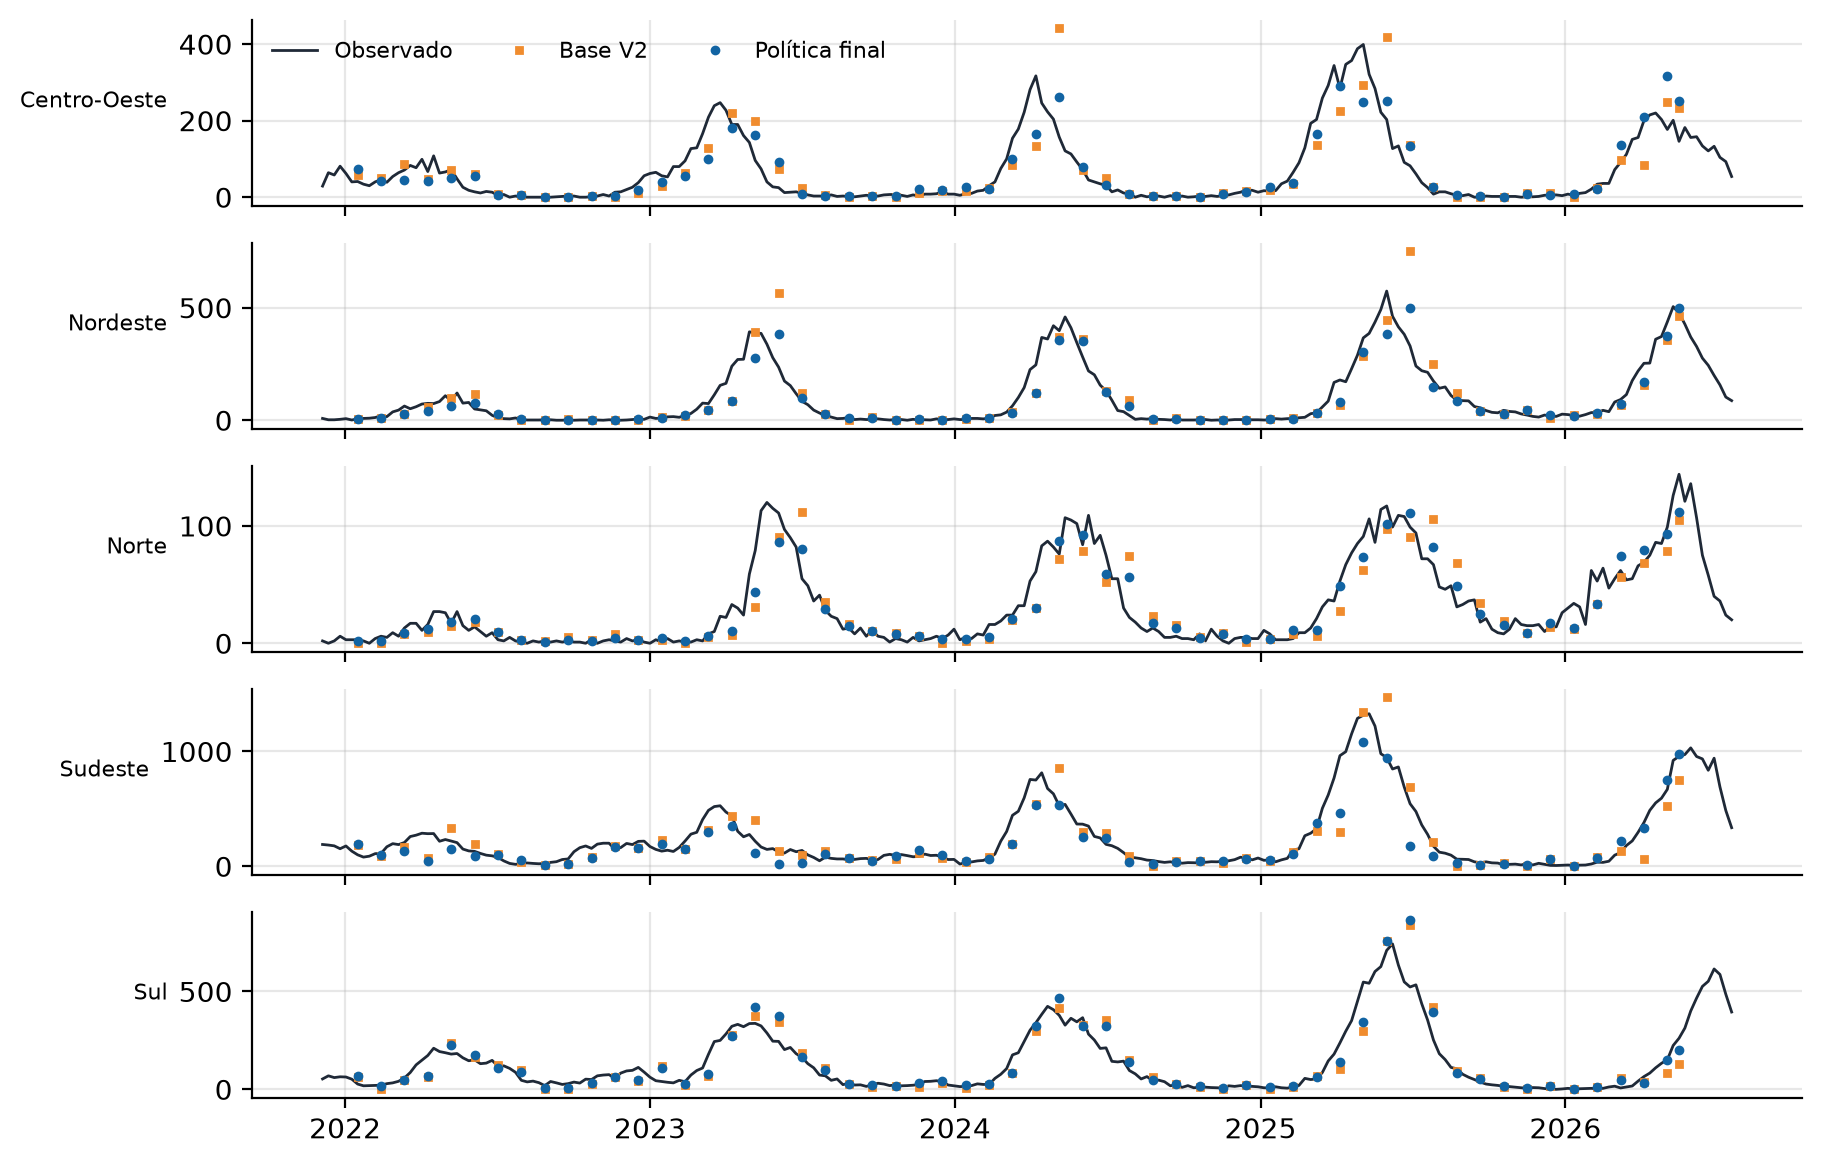
\includegraphics[width=\textwidth,height=.78\textheight,keepaspectratio]{regioes_obs_vs_prev_h4.png}
    \end{column}
    \begin{column}{.32\textwidth}
      \small
      \begin{itemize}
        \item As duas previsões ficam próximas; o MinT redistribui pouco entre regiões.
        \item O erro está concentrado nos picos: subida subestimada e descida superestimada (efeito de atraso).
        \item Norte, com picos mais largos, é o único beneficiado pelo MinT em $h=4$.
      \end{itemize}
    \end{column}
  \end{columns}
\end{frame}

% ===============================================================
\begin{frame}{UFs: o desempenho segue a intermitência}
  \begin{columns}[T,onlytextwidth]
    \begin{column}{.36\textwidth}
      \centering
      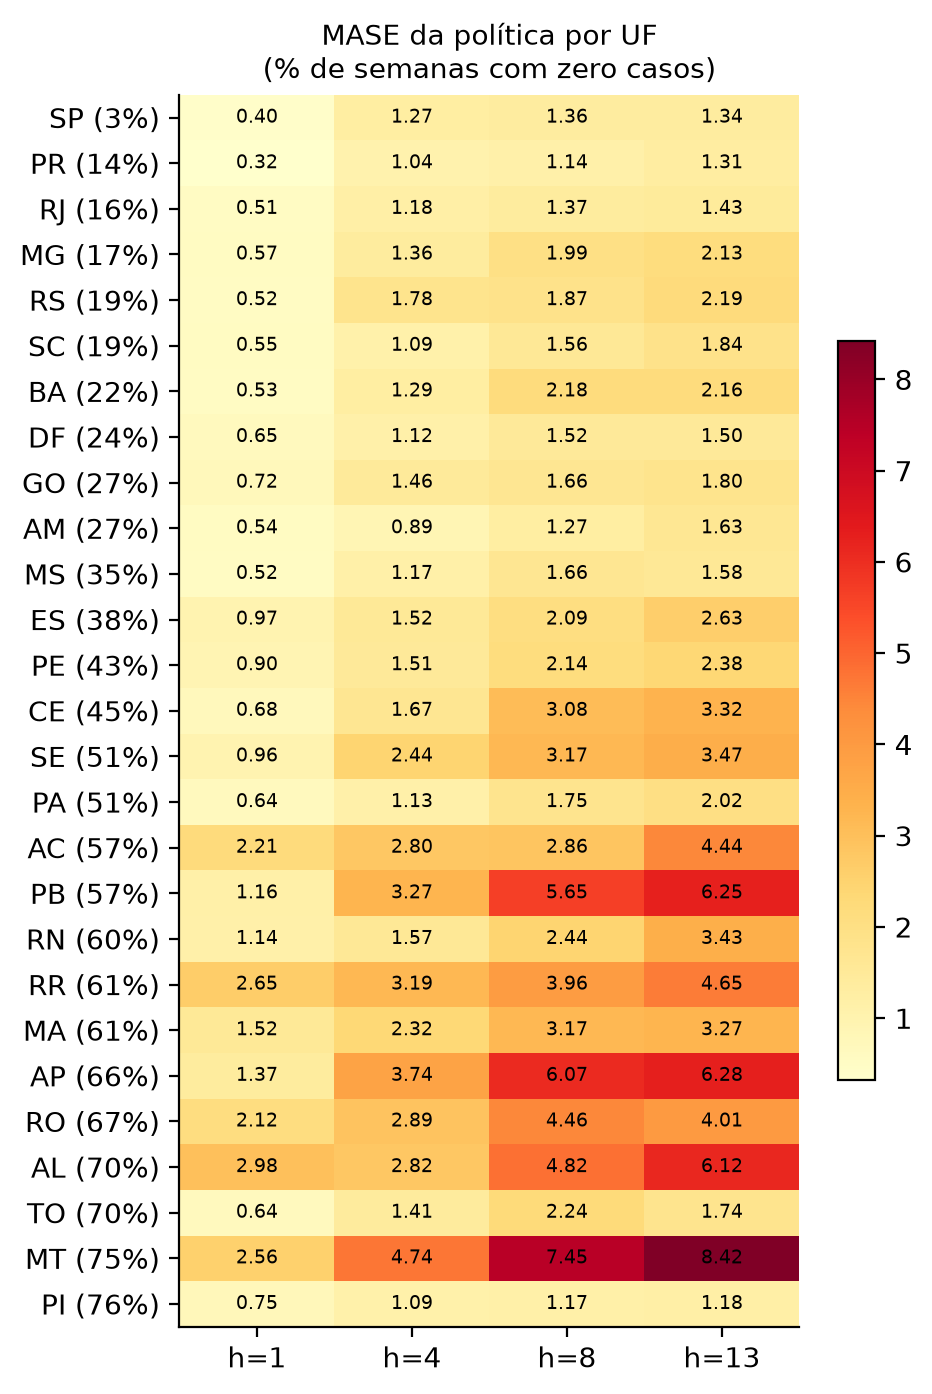
\includegraphics[height=.72\textheight]{ufs_mase_heatmap.png}
    \end{column}
    \begin{column}{.6\textwidth}
      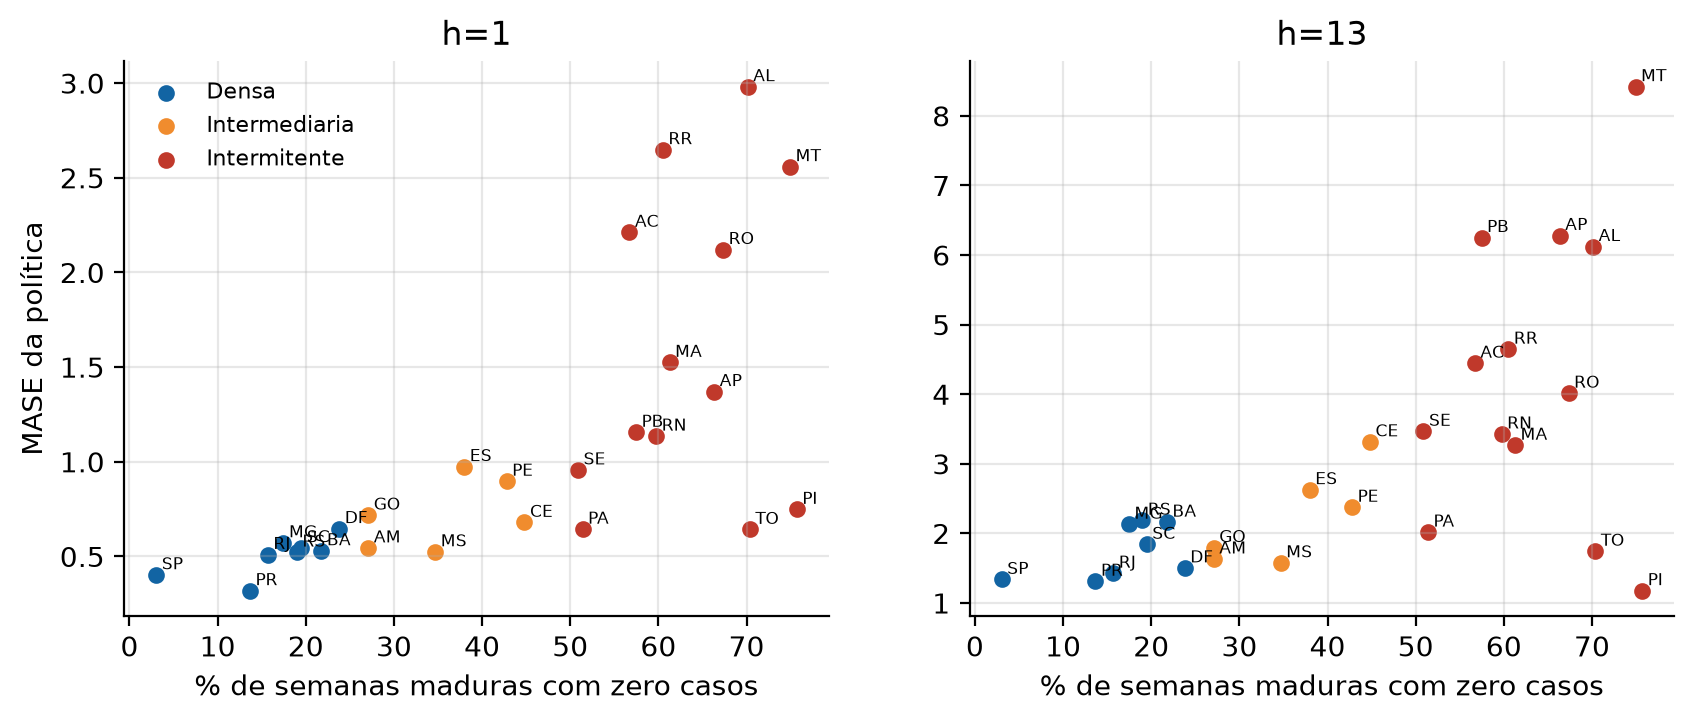
\includegraphics[width=.9\textwidth]{ufs_mase_vs_zeros.png}\par
      \small
      \begin{itemize}
        \item Correlação de 0,72 entre o MASE em $h=1$ e o \% de semanas com zero casos.
        \item Melhor UF: PR (0,36); pior: MT (2,99, 75\% de semanas zero).
        \item TO e PI têm MASE baixo apesar de muito intermitentes: quase sempre zero, e a previsão zero acerta.
      \end{itemize}
    \end{column}
  \end{columns}
\end{frame}

% ===============================================================
\begin{frame}{UFs: ganho do MinT não negativo sobre a Base V2}
  \begin{columns}[T,onlytextwidth]
    \begin{column}{.6\textwidth}
      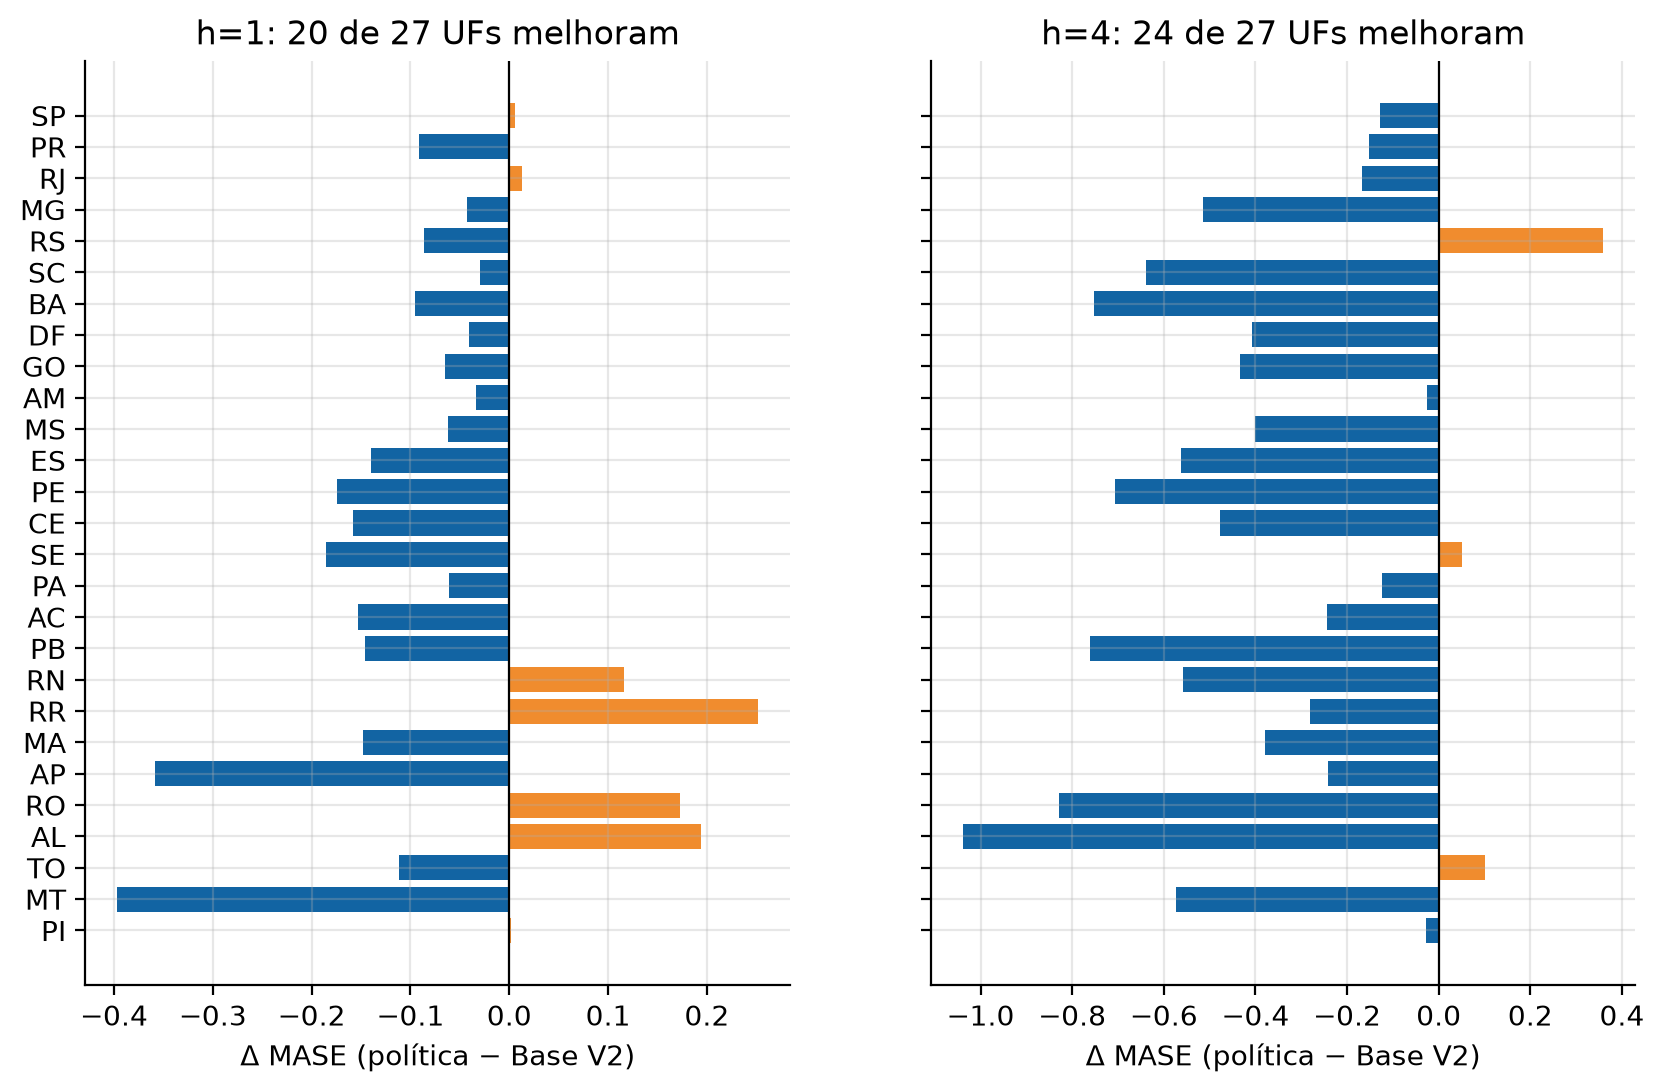
\includegraphics[width=\textwidth,height=.8\textheight,keepaspectratio]{ufs_delta_mint.png}
    \end{column}
    \begin{column}{.38\textwidth}
      \small
      \numero{17 de 27}{UFs melhoram em $h=1$ e em $h=4$ (azul).}
      \begin{itemize}
        \item Maiores ganhos em $h=4$: PE, AL, MA e BA ($\approx -0{,}4$). O sinal agregado do ETS corrige a persistência das UFs.
        \item Perdas: DF, TO, ES e MT. Em UFs quase sempre zero, a redistribuição adiciona casos que não ocorrem.
      \end{itemize}
    \end{column}
  \end{columns}
\end{frame}

% ===============================================================
\begin{frame}{Previsão operacional: Brasil a partir de 19/07/2026}
  \centering
  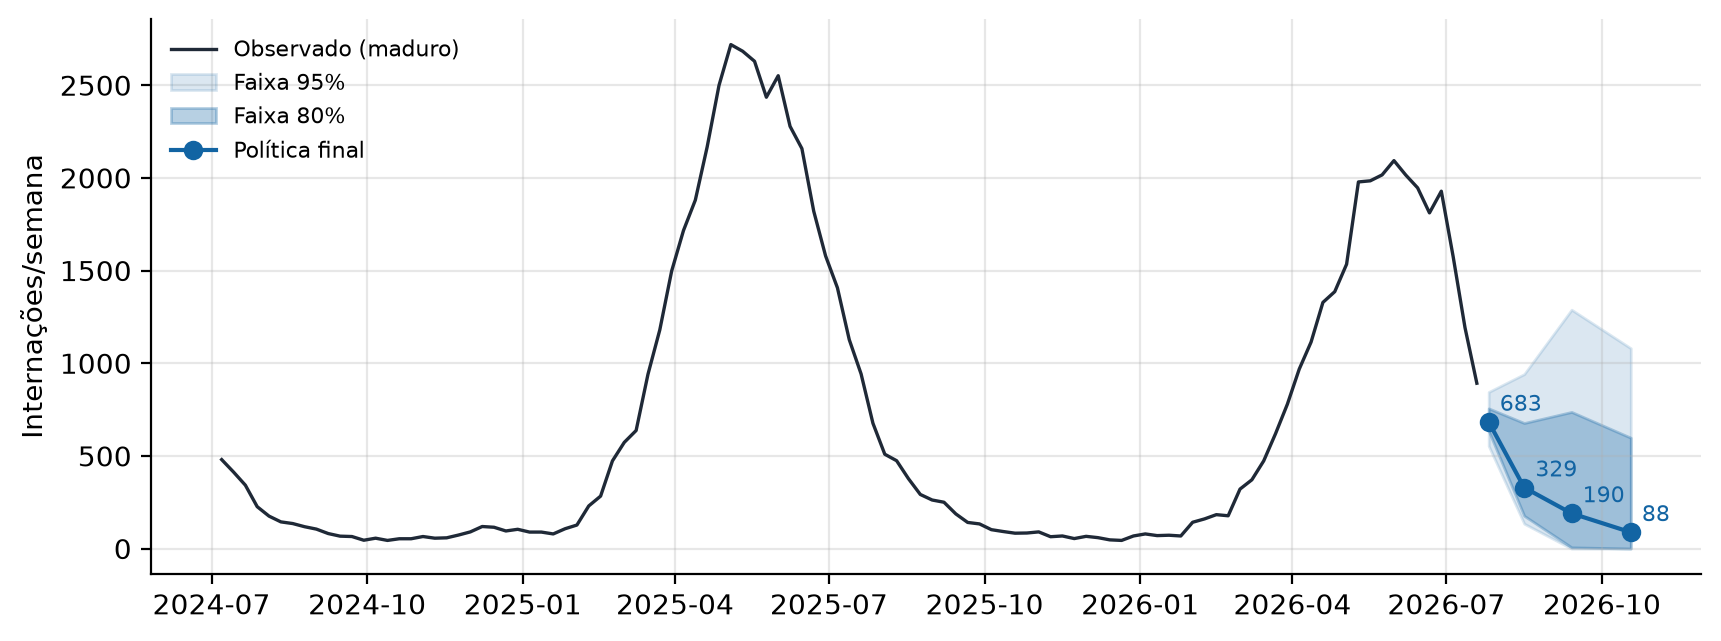
\includegraphics[width=.74\textwidth]{brasil_previsao_operacional.png}\par\vspace{2pt}
  \begin{columns}[T,onlytextwidth]
    \begin{column}{.5\textwidth}\small
      751 (80\%: 668--829) em 1 semana e 556 (268--914) em 4 semanas. Cobertura retrospectiva das faixas: 77--78\% (80\%) e 90--93\% (95\%).
    \end{column}
    \begin{column}{.46\textwidth}
      \begin{cartao}[borderline west={3pt}{0pt}{pucorange}]
        \footnotesize\textbf{Alerta:} o MinT ajustou o Brasil em +129 casos ($h=1$) e +551 ($h=4$), acima do máximo histórico. Comunicar como cenário sob alta discordância.
      \end{cartao}
    \end{column}
  \end{columns}
\end{frame}

% ===============================================================
\begin{frame}{Conclusões}
  \begin{columns}[T,onlytextwidth]
    \begin{column}{.55\textwidth}
      \begin{itemize}
        \item O horizonte domina o erro: MASE do Brasil vai de 0,33 ($h=1$) para cerca de 1,5 ($h\ge8$).
        \item A agregação ajuda: Brasil < regiões < UFs em todos os horizontes.
        \item Nas UFs, a intermitência explica a maior parte da dificuldade.
        \item O MinT não negativo transfere informação dos agregados para as UFs: ganha onde a previsão é mais difícil e cede pouco no Brasil.
      \end{itemize}
    \end{column}
    \begin{column}{.41\textwidth}
      \begin{mensagem}
        \small Para um boletim conjunto UF--região--Brasil, a política final entrega números coerentes e possíveis. Para um número nacional isolado de curto prazo, a Base V2 direta tem erro menor.
      \end{mensagem}
      \vspace{4pt}
      \nota{Próximo passo: avaliar a política congelada em semanas futuras maduras, fora dos 58 cortes usados na seleção.}
    \end{column}
  \end{columns}
\end{frame}

\end{document}
